\chapter{CUDA}

The problem this chapter aims to solve is implementing an aplication that is able to provide hierarchical clustering of very large datasets while retaining the reasonable computation time --- the time required to compute by a magnitude smaller datasets with current HCA algorithms.
Trying to achive this performance, we used a combination of C++ programming language and \textbf{CUDA}\footnote{Compute Unified Device Architecture.} API.

CUDA is a parallel platform with API allowing a programmer to use GPU for general purpose programming. This API exposes computational power of hundreds (even thousands) cores of CUDA-enabled GPUs \cite{cuda}.


\subsection{Terminology}

The starting point for running any code on GPU using CUDA is a \textbf{kernel}. A~kernel is a function that is executed on GPU; we say it contains \emph{device c code} is the phrase for code executed on CPU. Hence, a common CUDA application runs host code that determines which device code to run next. 

Kernel is run $n$ times in parallel by $n$ threads each having its unique \emph{thread ID}. IDs of threads can be identified by \emph{one-dimensional}, \emph{two-dimensional} or \emph{three-dimensional} indices forming block of threads, called \textbf{thread blode}. Complementary to a device code, a \emph{hostock}. This property reflects shapes of common structures such as vectors and matrices resulting in natural computation.

Since all block threads reside on the same processor and share common resources, the block size is limited\footnote{Currently up to 1024 threads.}. However, a kernel can be launched with multiple equally shaped blocks to increase the number of running threads. They can be organised into up to three-dimensional structure called \textbf{grid}. This naturally implies unique block ID. A grid can be of an arbitrary size; usually dictated by the computed data. It is a common practise that grid size surpasses the number of GPU processors.


\begin{figure}\centering
	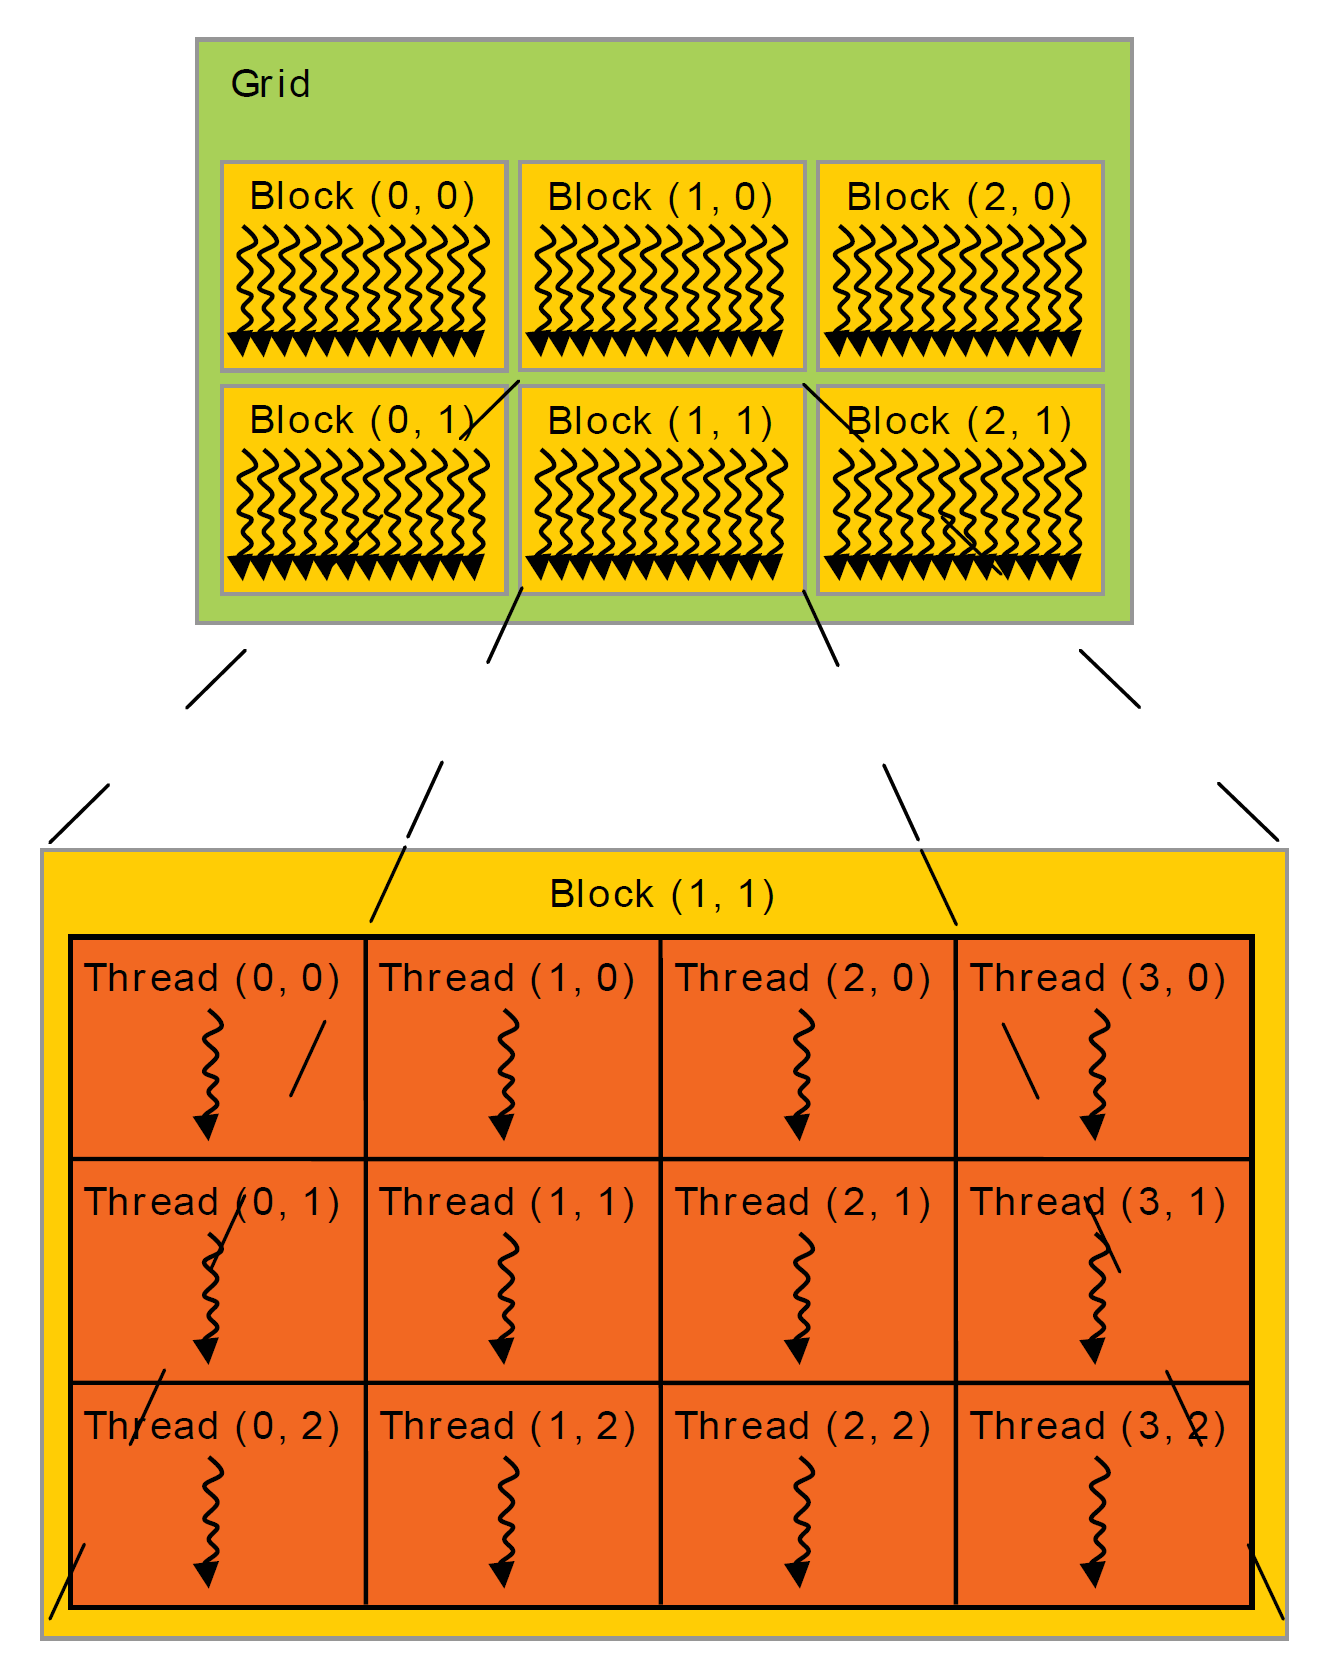
\includegraphics[width=7cm]{img/grid}
	\caption{Example of 2D grid of size (3,2) with 2D blocks of size (4,3).}
	\label{fig02:grid}
\end{figure}


The device memory is hierarchicaly divided into parts each being accessible by a different set of threads:

\begin{description}
	\item[Global memory] -- This memory is accessible by any thread. Any memory request is transfered via tranactions; hence, to avoid decrease of throughput, memory accesses should be coalesced. 
	\item[Local memory] -- Each thread has exclusive access to its local memory. Do not mislead this with registers, local memory is a private global memory.
	\item[Shared memory] -- Shared memory is assigned to a block, meaning that threads from the same block has access to the same shared memory. It is placed on-chip so it has much lower latency and higher bandwith than the global or local memory.
	\item[Constant memory] -- Read-only memory accesible by any thread. Due to its read-only property, it can be heavily cached and may perform better than global memory. Together with global memory, it persists across different kernel launches.
\end{description}

The building block of the CUDA-enabled GPU hardware architecture is multi-threaded \textbf{streaming multiprocessor (SM)}. GPU contains an array of multiprocessors whose number varies between different GPUs. When a kernel launches, its grid of blocks are distributed among available multiprocessors and execute in parallel (see fig \ref{fig02:SM}). On the selected multiprocessor, block threads are executed in parallel as well. Moreover, multiple blocks can run concurrently on one multiprocessor.

\begin{figure}\centering
 	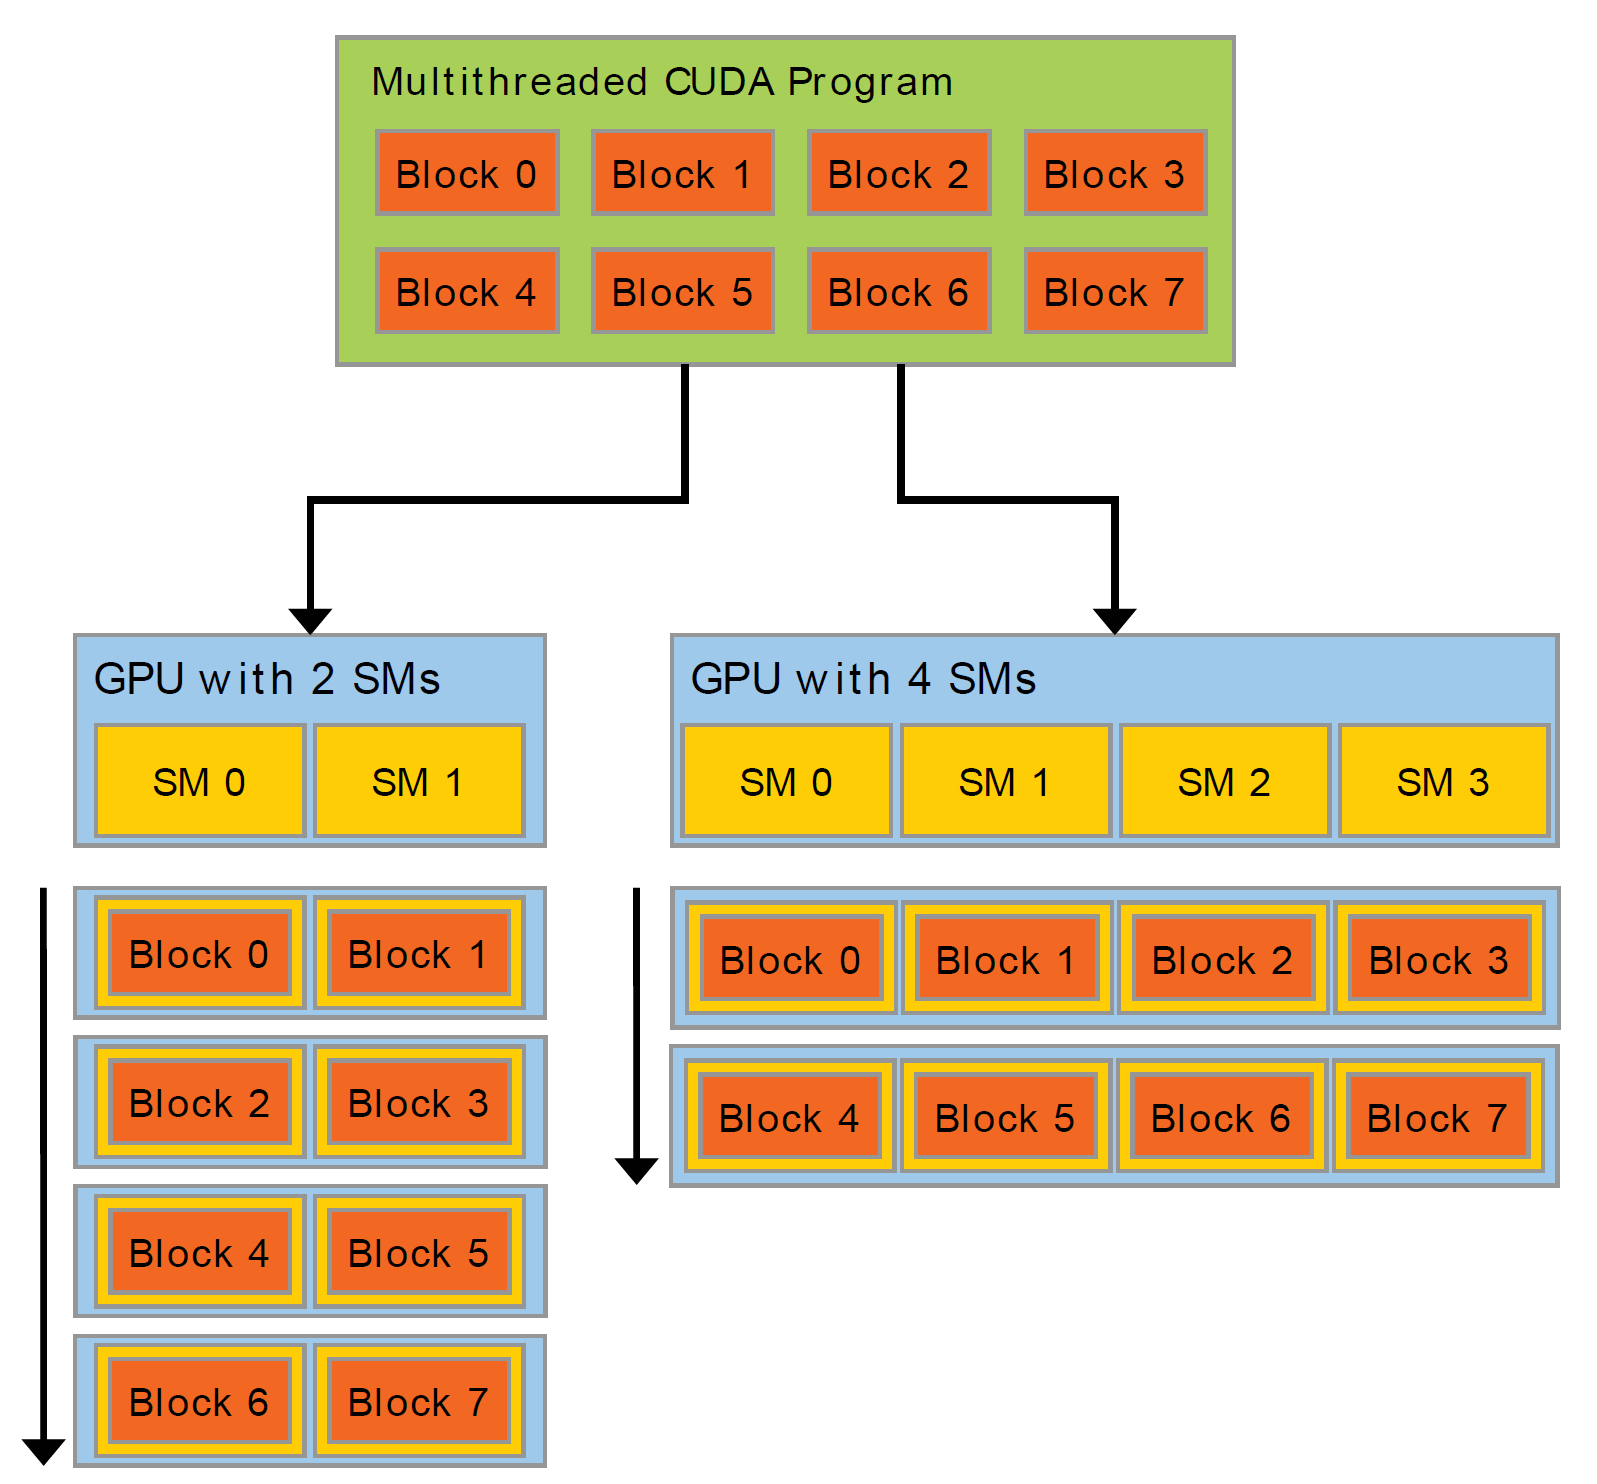
\includegraphics[width=8cm]{img/SM}
 	\caption{Example of different grid block distribution among SMs.}
 	\label{fig02:SM}
\end{figure}

To achieve this grade of parallelism, a GPU employs \textbf{SIMT\footnote{Single-Instruction Multiple-Threads.} architecture}. A multiprocessor partitions assigned block to chunks of 32 threads called \textbf{warps}. Each warp thread is executed concurrently. During the execution, threads start with the the same program address but have own registers and instruction pointers so they can branch independently. However, a warp executes one common instruction at the time. Hence, to achieve the greatest performance all warp threads must agree on the program path.
